\chapter{NEOS}

\red{need to rename the names everywhere for bce and neos}


\red{mention bandwidth somewhere 1e-8 und 0.2}

\red{shape uncertainties are always norm + shape, where?, hier weil resultat anwendung von histfactory }

\red{ttbar is negelected because}

\red{also say here we havent done any optimization on neos}

\red{add correlation mjj etajj}

\red{adapt variable selection writing}

\red{too tight slope not good, or neos methdos part?}

\red{bandwidth choice, sensitive to bandwidth and slope}

This chapter compares the \ac{neos} approach to established methods by evaluating upper cross-section limits on the boosted \ac{vbf} $HH\rightarrow4b$ analysis. This evaluation employs \ac{neos} in what this thesis terms `autoanalysis', wherein only the most basic selections of reconstructed objects that encapsulate the process of interest are used, and \ac{neos} optimizes considered cuts and uncertainties simultaneously when searching for the best limits. The objective here is not to find the most stringent cross-section limits but to provide a fair comparison and present the potential \ac{neos} offers compared to more traditional methods.

Cross-section upper limits are obtained with a maximum likelihood fit as explained in chapter \ref{sec:statistics}. \ac{neos} is compared against limits from using the Higgs pair invariant mass $m_{HH}$ and a classifier \ac{nn} trained on separation for signal to background with a \ac{bce} loss function as of equation \ref{eq:bce}. Models are trained with the \ac{tomatos} \ac{nn} training framework developed for this purpose \citep{tomatos} described in section \ref{sec:neos_training}. Both the training for \ac{neos} as well as the classifier use the same \ac{nn} architecture described in \ref{sec:event_classification}, and the hyperparameters are kept consistent to ensure a fair comparison.

Each fit employs the same subset of uncertainties, chosen from the highest-ranked uncertainties of an $m_{HH}$ fit that incorporated the full set of uncertainties. The reduced set used in optimizing \ac{neos} is summarized in table \ref{tab:neos-samples} and ranked by its impact on an \mhh fit illustrated in Figure \ref{fig:m_hh_neos_unc_ranking} \red{replace with ps}. The complete ranked list of uncertainties on the \mhh fit is available in Appendix \ref{fig:m_hh_full_sys_ranking}. To demonstrate compatibility across all types of uncertainties, both nominal statistical uncertainties and two jet-related uncertainties are included. The \ac{pdf}+$\alpha_s$ uncertainty, however, was excluded from the optimization due to its minimal impact relative to the computational overhead of processing 100 additional samples.


\begin{figure}
    \centering
    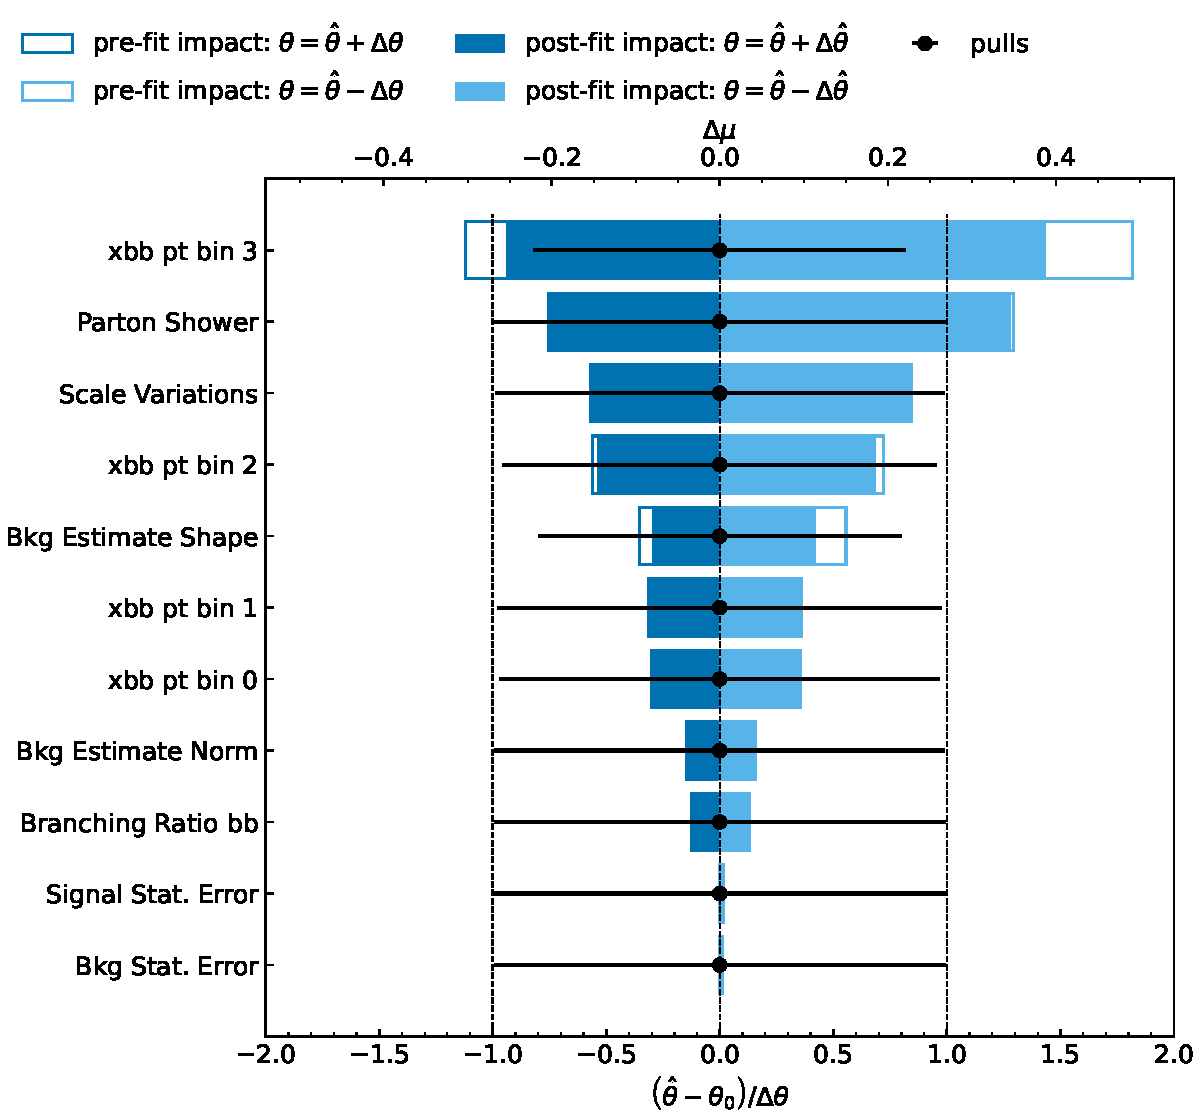
\includegraphics[width=0.95\textwidth]{neos_results/m_hh_neos_unc_ranking.pdf}
    \caption[]{Ranking of nuisance parameters ordered by their post-fit impact on the signal strength, $\Delta\mu$, displayed on the upper axis for an invariant Higgs Pair mass fit (\mhh{}). The impact of a nuisance parameter $\Theta$ is assessed by performing four fits. In each fit, the parameter $\Theta$ is fixed to its nominal best-fit value $\hat{\Theta}$ plus a given nuisance parameter uncertainty $\Delta\Theta$. The difference between the resulting fitted signal strength $\mu_\text{fit}$ and the nominal best-fitted value is then computed as $\Delta\mu=\hat{\mu} - \mu_\text{fit}$. This process is repeated for pre-fit $\pm\Delta\Theta$ and post-fit $\pm\Delta\hat{\Theta}$ uncertainties of $\Theta$. The lower axis and the black points represent the pull for each nuisance paramter, calculated as the difference between the best-fit value and the nominal pre-fit $(\hat{\Theta} - \Theta_0)$, divided by its variance $\Delta\Theta$ for the parameter $\Theta$. If the model is accurate, the expected value of each pull should be zero, with a variance of one, in the asymptotic limit. In this limit the test statistic is computed from the sum of pulls and follows a $\chi^2$ distribution if the model is correct. Therefore, pulls serve as goodness-of-fit quantities. }
    \label{fig:m_hh_neos_unc_ranking}
\end{figure}

\section{Training}
The $\ktwov=0$ sample is used due to its large statistic as nominal \ac{vbf} signal sample. Figure \ref{fig:training_metrics_validation} presents the training loss and Asimov significance per epoch and as well histograms of the final model evaluated on the samples from table \ref{tab:neos-samples} for both the \ac{bce}-trained \ac{nn} and the neos \ac{nn}. While the loss function for the classifier converges for the validation dataset at about epoch 400, the \cls loss evaluation shows strong signs of overfitting starting at epoch $\sim$200. Even though the smallest validation loss is at the last epoch, limits determined using the \ac{nn} from the local minimum epoch 185 gained better results and is thus chosen for \ac{neos}. The best validated epoch for the \ac{bce}-trained \ac{nn} 993. The score of the \ac{bce}-trained \ac{nn} exhibits the typical feature of classifier separation, with most of the background in the lowest bin and decreasing event counts in higher bins. When evaluated on signal samples, the behavior is reversed, with the largest impact of uncertainties on the signal occurring in the last bin. A different behavior can be observed in the histogram of the \ac{neos} approach. The signal sample is more spread over all bins and since a maximum likelihood fit exhibits a mirror symmetry on the given histograms the results can be inverted labeling for the \ac{nn} score. Furthermore, the Asimov significance, as defined in equation \ref{eq:asimov-significance}, commonly used as a proxy for statistical testing during analysis optimization, shows no clear correlation with the \ac{bce}-trained \ac{nn}. In contrast, it anti-correlates with the \ac{neos} loss function, hinting at a potential advantage of the neos approach.

\begin{figure}
    \centering
    \subfigure[]{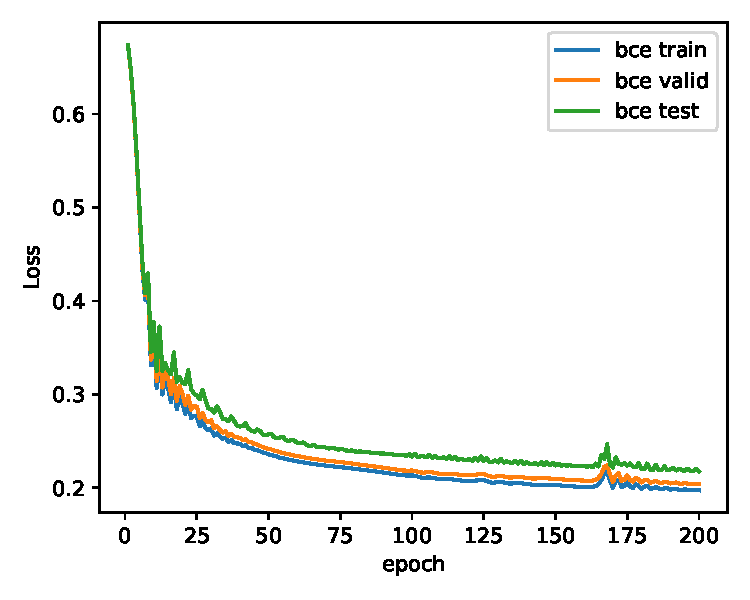
\includegraphics[width=.45\textwidth]{neos_results/tomatos_bce_5_1000/bce.pdf}}
    \subfigure[]{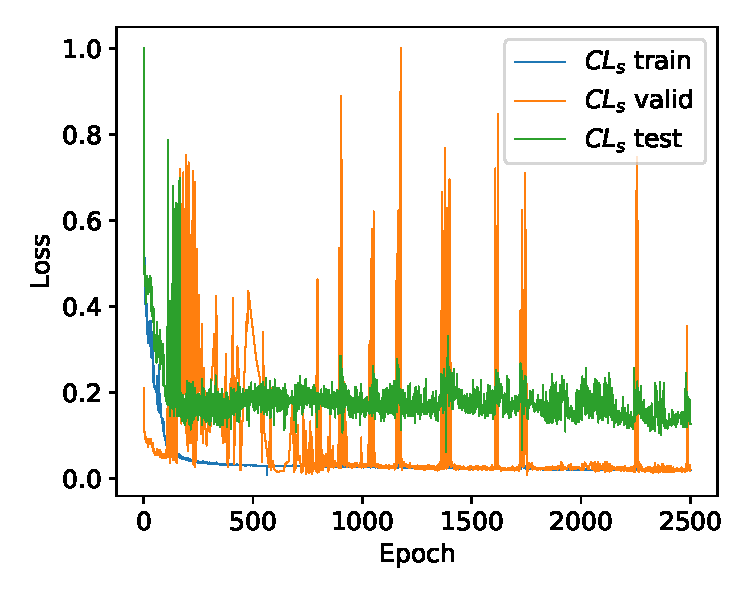
\includegraphics[width=.45\textwidth]{neos_results/tomatos_cls_5_2500_slope_50/cls.pdf}} \label{fig:neos_validation_loss}\\
    \subfigure[]{\includegraphics[width=.45\textwidth]{neos_results/tomatos_bce_5_1000/hist.pdf}}
    \subfigure[]{\includegraphics[width=.45\textwidth]{neos_results/tomatos_cls_5_2500_slope_50/hist.pdf}} \\
    \subfigure[]{\includegraphics[width=.45\textwidth]{neos_results/tomatos_bce_5_1000/Z_A.pdf}}
    \subfigure[]{\includegraphics[width=.45\textwidth]{neos_results/tomatos_cls_5_2500_slope_50/Z_A.pdf}} \\
    \caption[]{\textbf{(Left Column)} \ac{nn} trained with a \ac{bce} loss function. \textbf{(Right Coloumn)} \ac{nn} trained with \ac{neos}.  \textbf{(Top To bottom)}: Loss function evaluated on training, validation and test dataset per training epoch, histogrammed \ac{nn} score for samples used in the training and Asimov significance. }
    \label{fig:training_metrics_validation}
\end{figure}


% \begin{figure}
%     \centering
%     \subfigure[]{
\includegraphics[width=.47\textwidth]{red}}
%     \subfigure[]{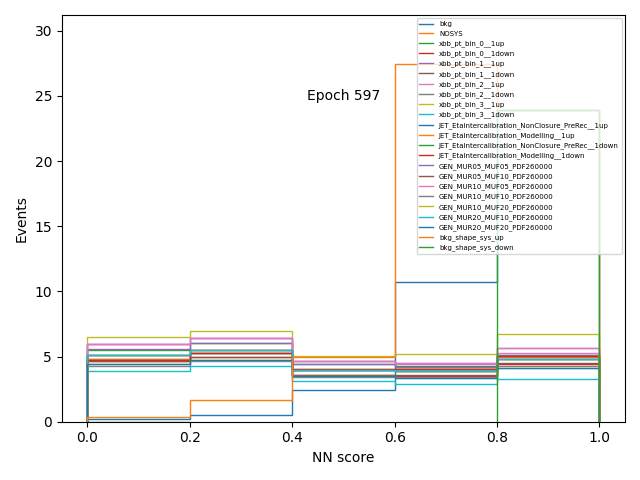
\includegraphics[width=.47\textwidth]{neos_results/tomatos_cls_5_2500_slope_50/images/0597.png}}
%     \caption[]{\red{(a)bce (b)cls Histograms used in the optimization after Kernel Density Estimation. hyperparameter tweaking it looses gradient if I go below bandwidth 0.2 }}
%     \label{fig:neos_valid_kde_hists}
% \end{figure}


\subsection{Background Estimate Optimization}
As can be seen from the uncertainty ranking the background estimate shape uncertainty is one of the crucial uncertainties in this analysis. Since \ac{neos} controls the histogram shape of the \ac{nn} score it can effectively reduce this uncertainty. Figure \ref{fig:neos_valid_bkg_shape_sys} depicts the relative error to the nominal background during training with the minimum close to epoch 185 found by the validation loss. The observed instability after epoch 200 is potentially due to overtraining. The instability observed up to epoch 200 could be the result of an excessively small gradient, which might be mitigated by artificially increasing the gradient for this uncertainty during training.
\begin{figure}
    \centering
    \subfigure[]{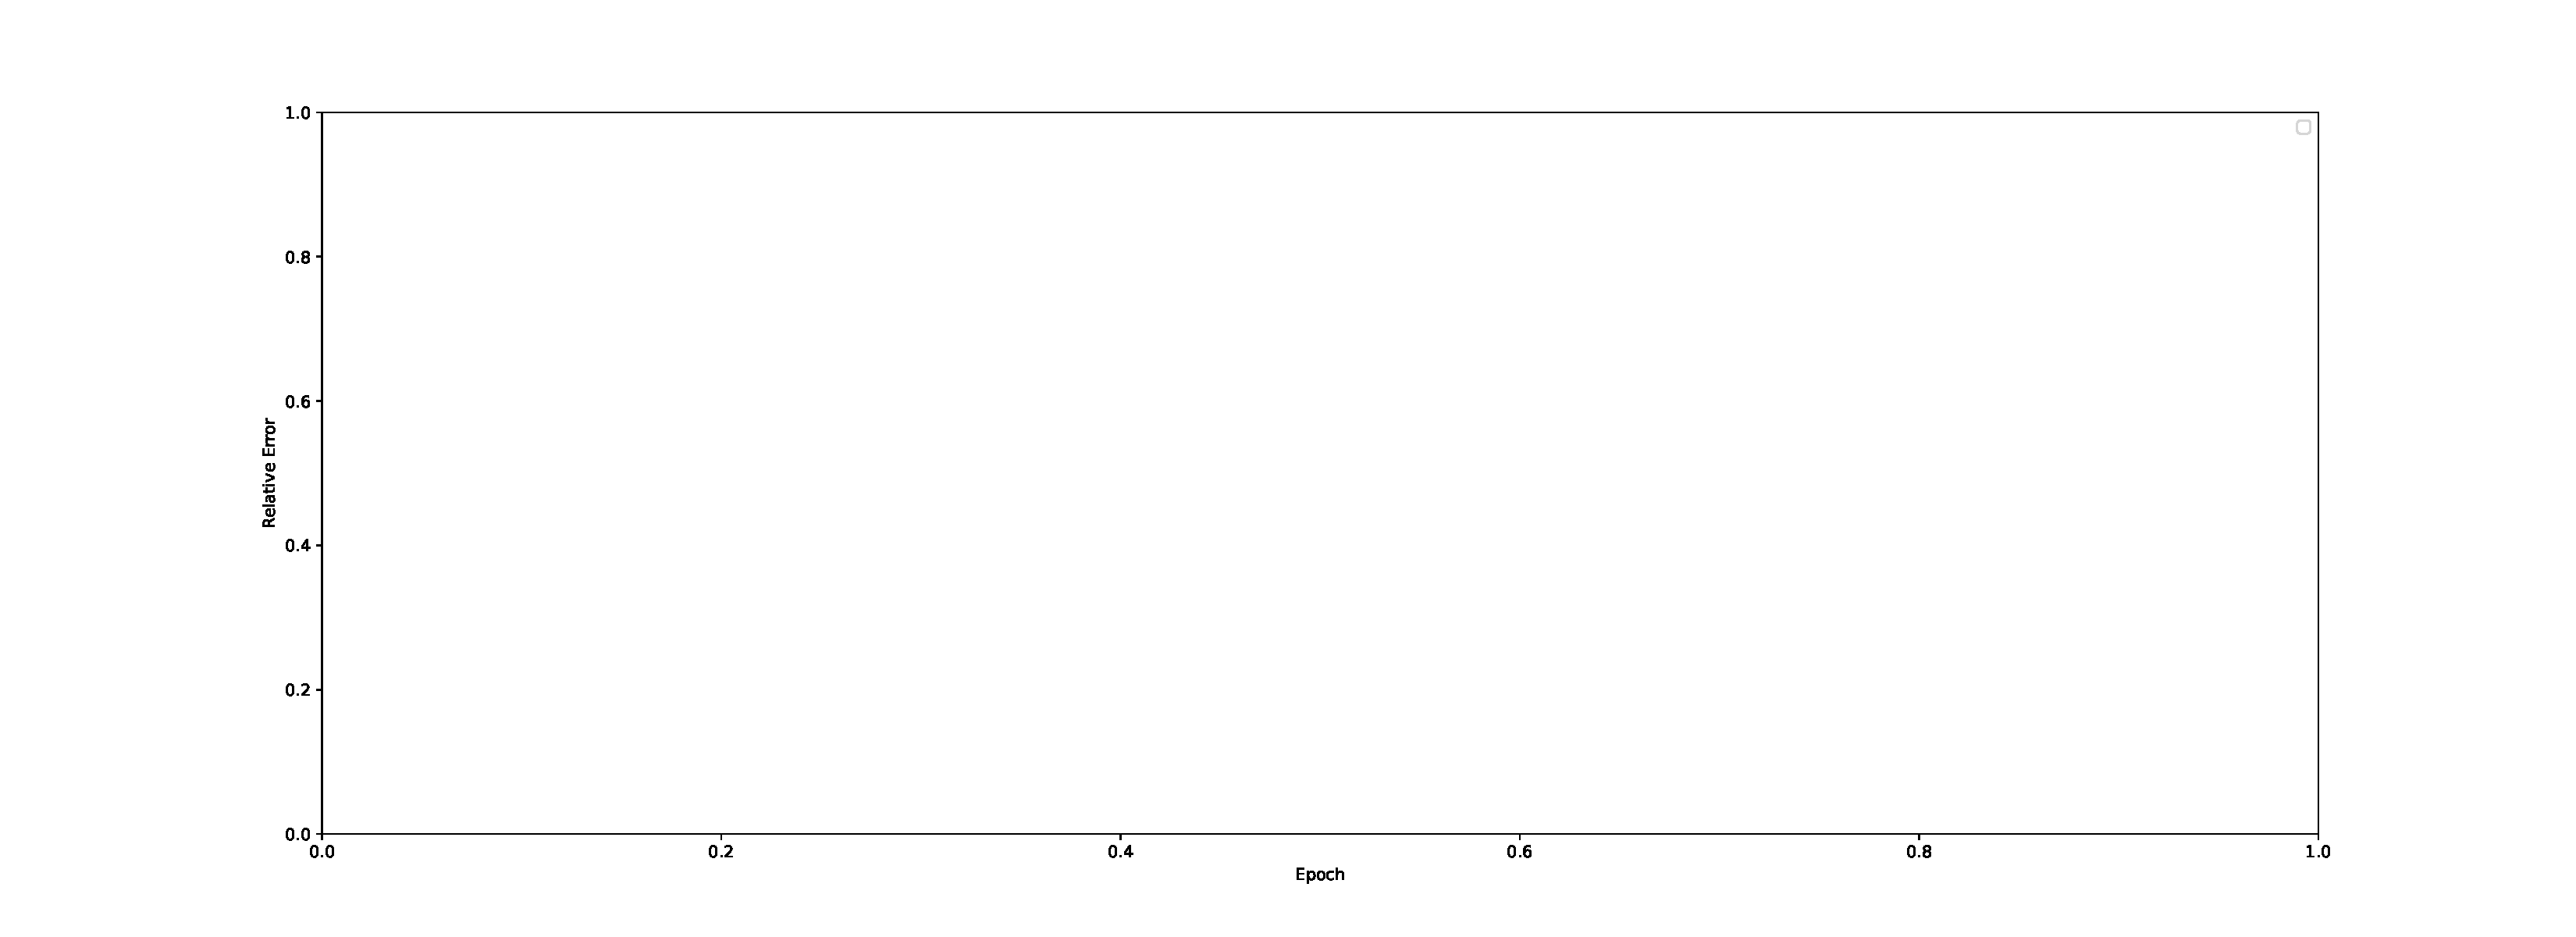
\includegraphics[width=.97\textwidth]{neos_results/bkg_shape_sys_rel_error.pdf}}\\
    \subfigure[]{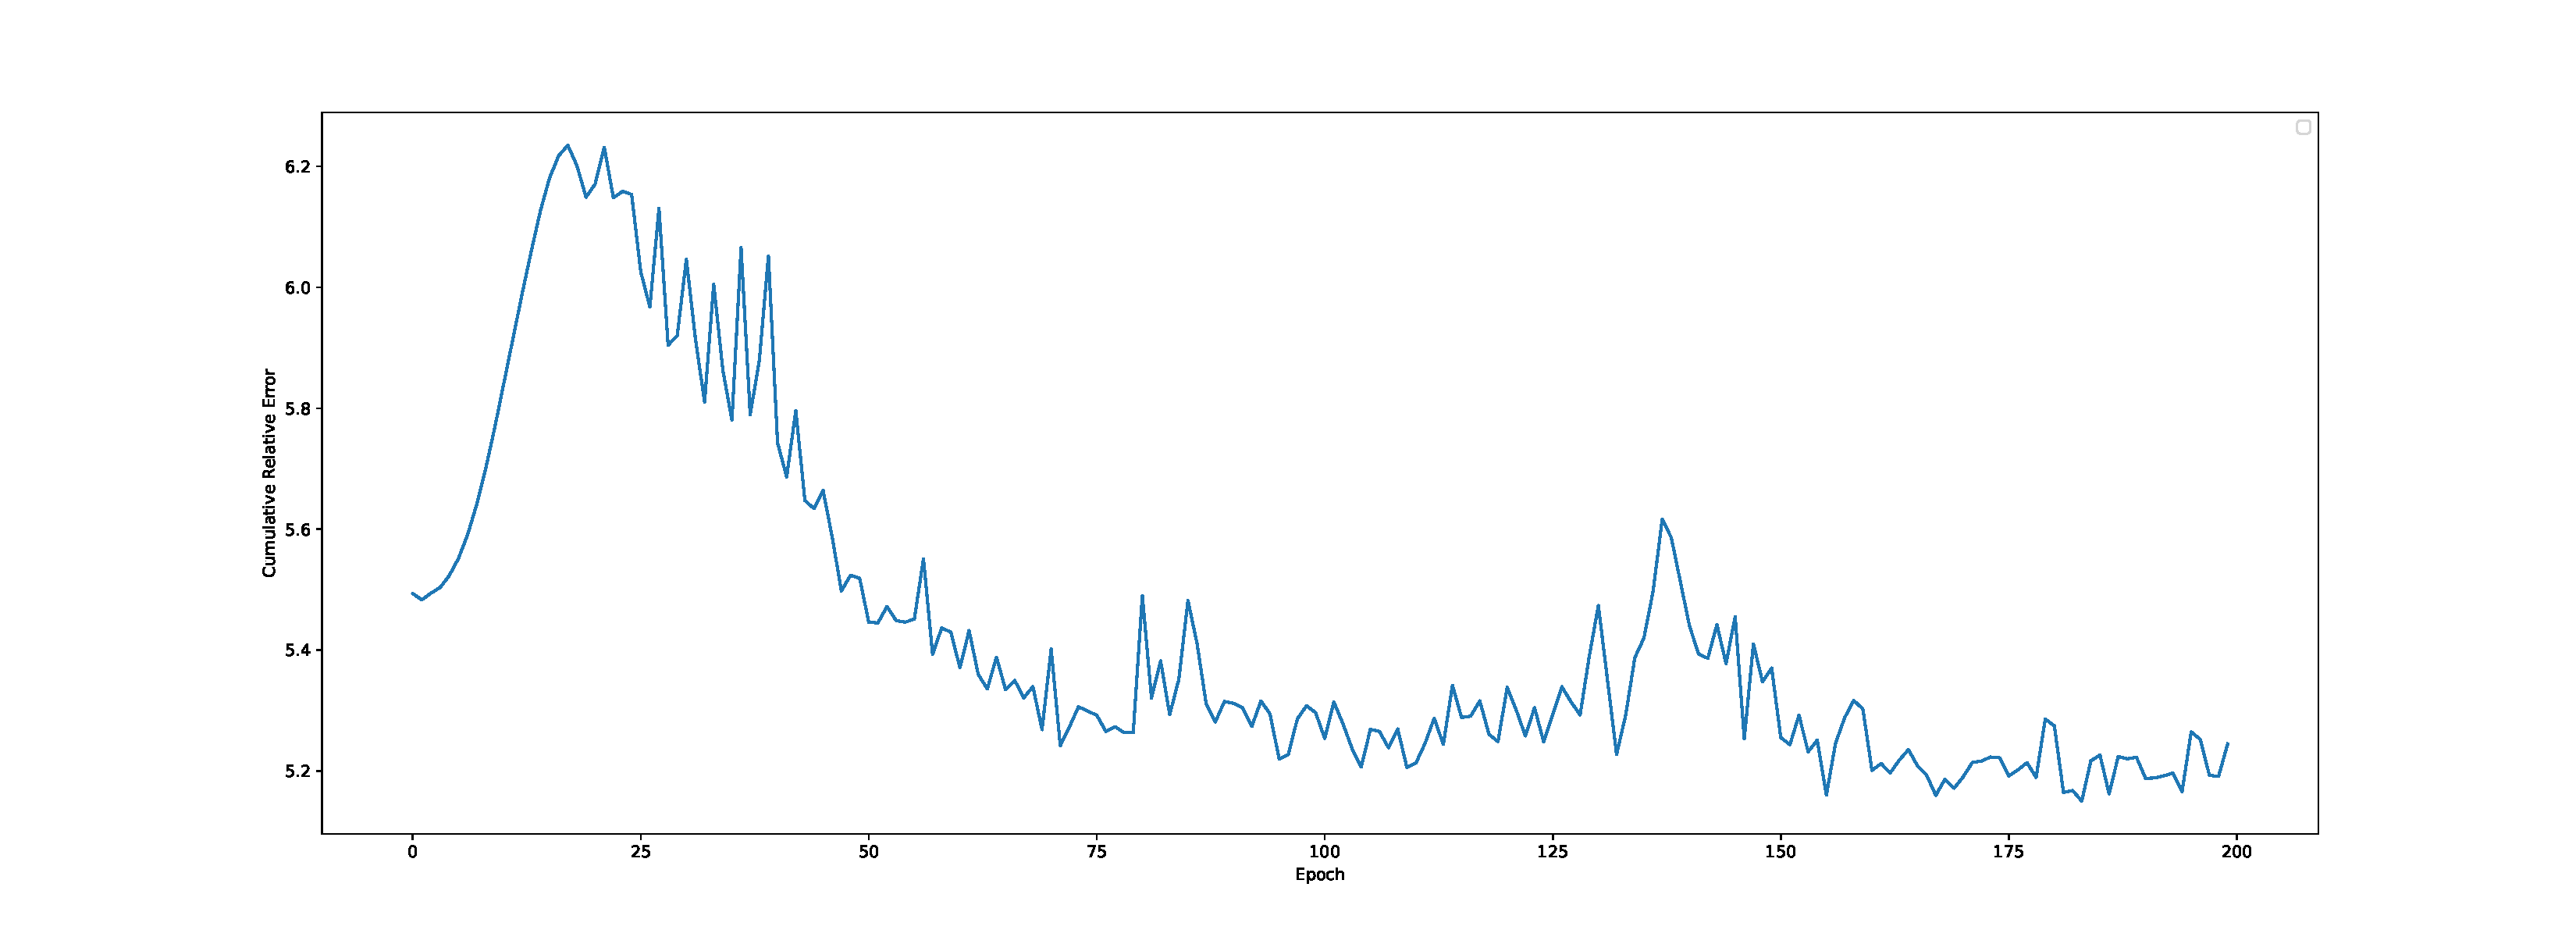
\includegraphics[width=.97\textwidth]{neos_results/bkg_shape_sys_rel_error_cumulative.pdf}}
    \caption[]{Relative error of the background shape uncertainty to the nominal background estimate (a) per bin and (b) summed across all bins.}
    \label{fig:neos_valid_bkg_shape_sys}
\end{figure}

\subsection{Cuts Optimization}
To determine the $m_{jj}$ and $|\Delta\eta(j,j)|$ cuts on the \ac{vbf} jets for the \mhh and \ac{bce}-trained \ac{nn}, cuts are scanned and the resulting histogram is evaluated on the Asimov significance. Figure \ref{fig:cut_scan} presents the results of this procedure depending on the cuts and table \ref{tab:z_a_cuts} displays the derived cuts from maximizing the Asimov significance. \ac{neos} is also included in the procedure for comparison purposes. Cuts found by the \ac{neos} optimization as explained in \ref{sec:neos_training} are shown in figure \ref{fig:neos_cuts} and display a major feature of training \ac{neos} including cuts at this stage.

Loosening a cut corresponds to introducing new data which is always beneficial in training \acp{nn} and thus results in a smaller training loss. However at the same time it is not obvious how uncertainties like the background estimate are affected by this change. Ideally \ac{neos} should be able to capture this but the instability of the training loss indicates a hard to find gradient for \ac{neos} for this procedure. This also potentially explain the shape of the validation loss for the \ac{neos} training as of figure \ref{fig:neos_validation_loss}. Overtraining starts around epoch 200 and worsens until epoch 400 which is where the cuts merely change. Upon introducing more data by further loosening the cuts around epoch 400 the validation also decreases again until at epoch 600 where $m_{jj}$ plateaus again. However the \ac{nn} is potentially already in a local overtrained minimum showing no signs of further improvement and the training becomes unstable. \red{This is further investigated in chapter \ref{ch:hh4b-results}.}

\red{say also again about asimov for neos eta probably too tight for bkg estimate}

\begin{figure}
    \centering
    \subfigure[]{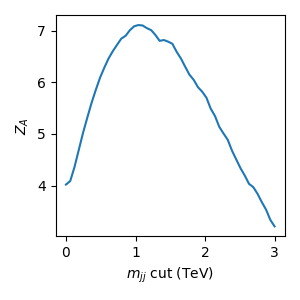
\includegraphics[width=.3\textwidth]{s_b_optimization/s_b_optimization_m_hh_5_m_jj}}
    \subfigure[]{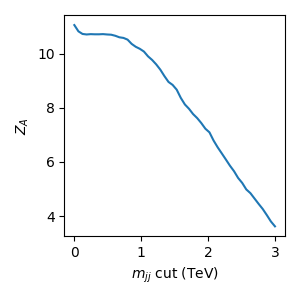
\includegraphics[width=.3\textwidth]{s_b_optimization/s_b_optimization_tomatos_bce_5_1000_m_jj}}
    % \subfigure[]{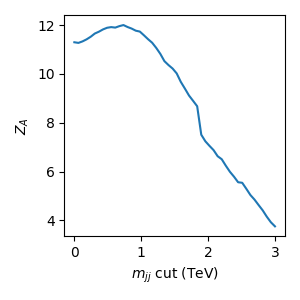
\includegraphics[width=.3\textwidth]{s_b_optimization/s_b_optimization_tomatos_cls_5_2500_slope_50_m_jj}}\\
    \subfigure[]{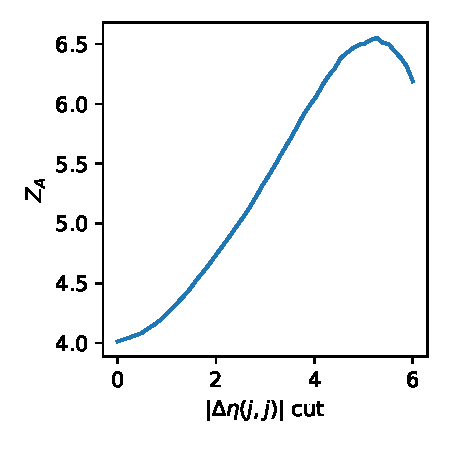
\includegraphics[width=.3\textwidth]{s_b_optimization/s_b_optimization_m_hh_5_eta_jj}}
    \subfigure[]{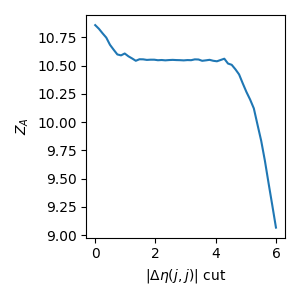
\includegraphics[width=.3\textwidth]{s_b_optimization/s_b_optimization_tomatos_bce_5_1000_eta_jj}}
    % \subfigure[]{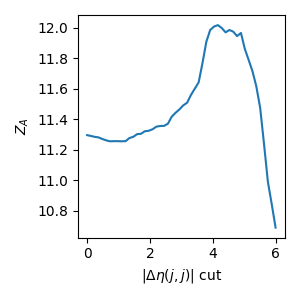
\includegraphics[width=.3\textwidth]{s_b_optimization/s_b_optimization_tomatos_cls_5_2500_slope_50_eta_jj}}
    \caption[]{Columns left to right: $\mhh$, \ac{bce}-trained \ac{nn}, \ac{neos}-trained \ac{nn}: Asimov Significances after applying a cut on \textbf{(a)-(c)} on the invariant mass $m_{jj}$ and \textbf{(d)-(f)} the pseudorapidity separation $|\Delta\eta(j,j)|$ of the \ac{vbf} jets. \red{redo}}
    \label{fig:cut_scan}
\end{figure}

\begin{figure}
    \centering
    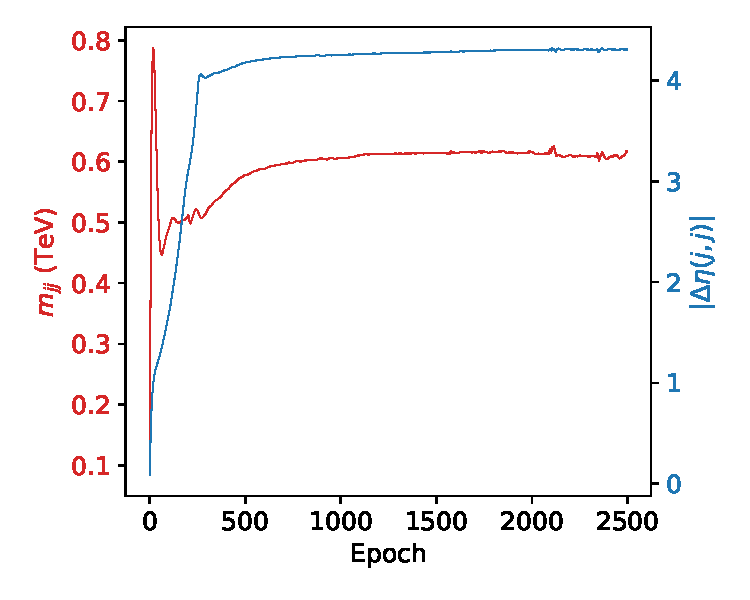
\includegraphics[width=.6\textwidth]{neos_results/tomatos_cls_5_2500_slope_50/cuts}
    \caption[]{Optimized \ac{neos} cuts per epoch for the invariant mass $m_{jj}$ and the pseudorapidity difference $|\Delta\eta(j,j)|$ of the two \ac{vbf} jets.}
    \label{fig:neos_cuts}
\end{figure}

\begin{table}[htbp]\label{tab:z_a_cuts}
    \centering
    \caption{Optimized cuts for \mhh and the trained \acp{nn} from the maximized Asimov significances shown in figure \ref{fig:cut_scan} and the cuts found by the \ac{neos} optimization in epoch 185 of figure \ref{fig:neos_cuts}.}
    \begin{tabular}{c|c|c}
                                  & $m_{jj}$ (GeV) & $|\Delta\eta(j,j)|$ \\\hline
        \mhh                      & >1041          & >5.27               \\
        \ac{bce}-trained \ac{nn}  & >0             & >0                  \\
        \ac{neos}-trained \ac{nn} & >673           & >4.29               \\ \hline
        \ac{neos} (epoch 185)     & >481           & >1.45               \\
    \end{tabular}
\end{table}



\section{Performance Comparison}
After training the \acp{nn} they are evaluated alongside an $\mhh$ fit without the use of any \ac{neos} methods to determine limits on the boosted \ac{vbf} $HH\rightarrow4b$ cross-section with the \textit{cabinetry} fitting framework \citep{cranmer_2021_4627038}. Hence, the event selection, application of found cuts or the creation of histograms are applied traditionally.

All models use the same methods for the background uncertainty estimation described in \ref{sec:bkg_uncertainties}. Uncertainties used for the fitting are shown in figure \ref{fig:neos_validation_uncertaintes_1} and \ref{fig:neos_validation_uncertaintes_2}. \ac{ggf} signal uncertainties are omitted here as the difference of adding the \ac{ggf} signal to the fitting procedure has a \qty{1}{\percent}(\qty{0.5}{\percent}) impact on the cross-section limits when using the \ac{sm}($\ktwov=0$) \ac{vbf} signal in the maximum likelihood fit.


\begin{figure}
    \centering
    \subfigure[]{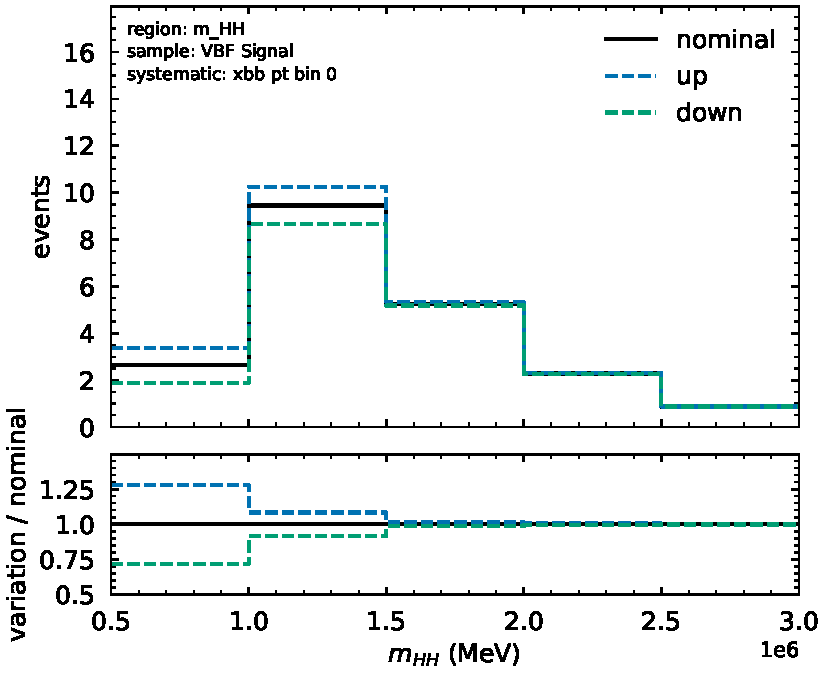
\includegraphics[width=.3\textwidth]{neos_results/m_hh_5_l1cvv0cv1/figures/templates/m_HH_VBF-Signal_xbb-pt-bin-0.pdf}}
    \subfigure[]{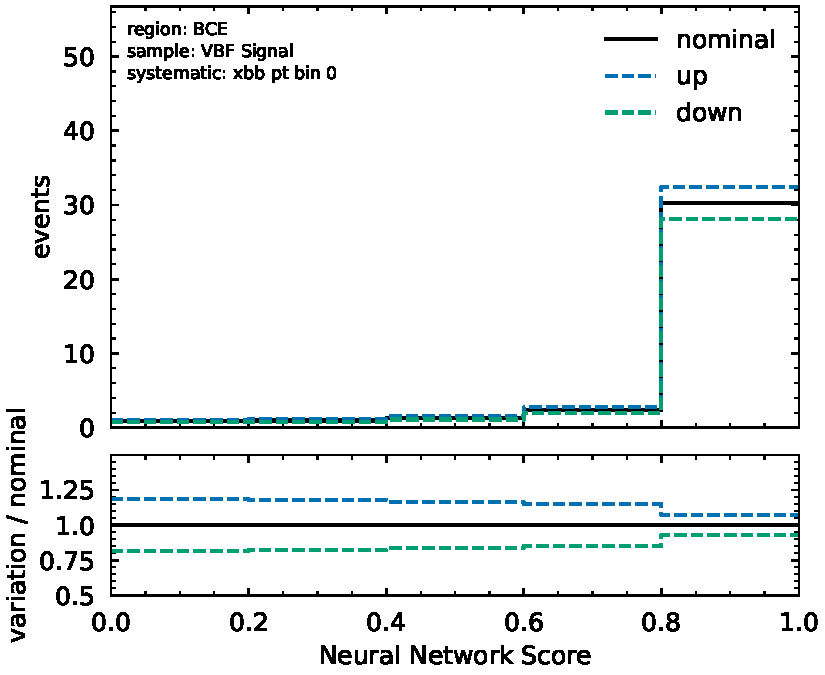
\includegraphics[width=.3\textwidth]{neos_results/tomatos_bce_5_1000_l1cvv0cv1/figures/templates/BCE_VBF-Signal_xbb-pt-bin-0.pdf}}
    \subfigure[]{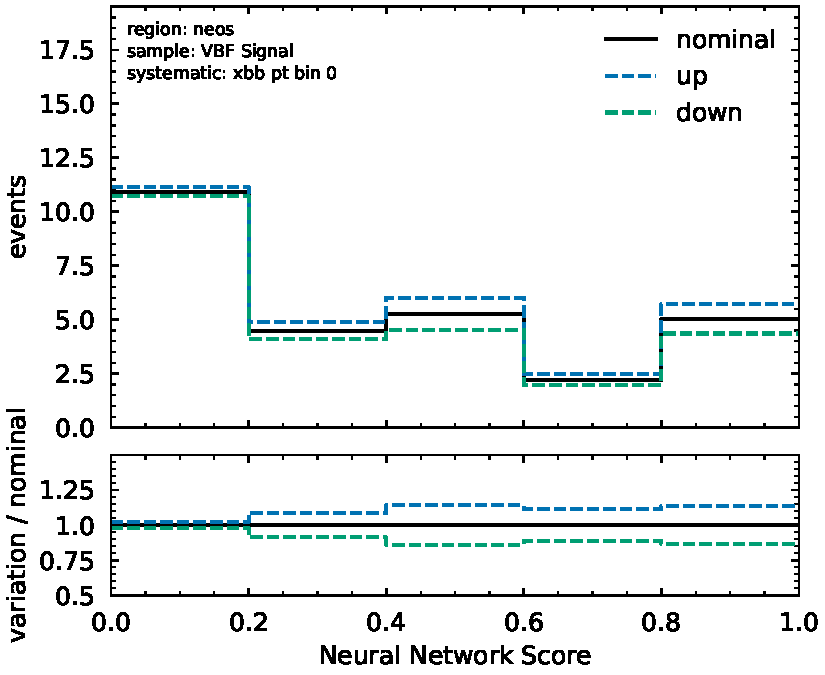
\includegraphics[width=.3\textwidth]{neos_results/tomatos_cls_5_2500_slope_50_l1cvv0cv1/figures/templates/neos_VBF-Signal_xbb-pt-bin-0.pdf}} \\
    \subfigure[]{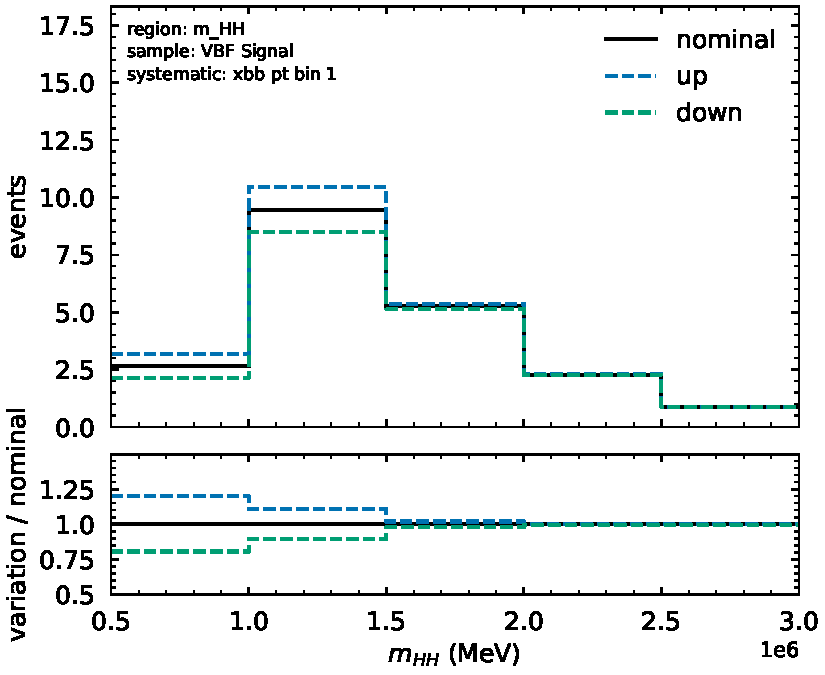
\includegraphics[width=.3\textwidth]{neos_results/m_hh_5_l1cvv0cv1/figures/templates/m_HH_VBF-Signal_xbb-pt-bin-1.pdf}}
    \subfigure[]{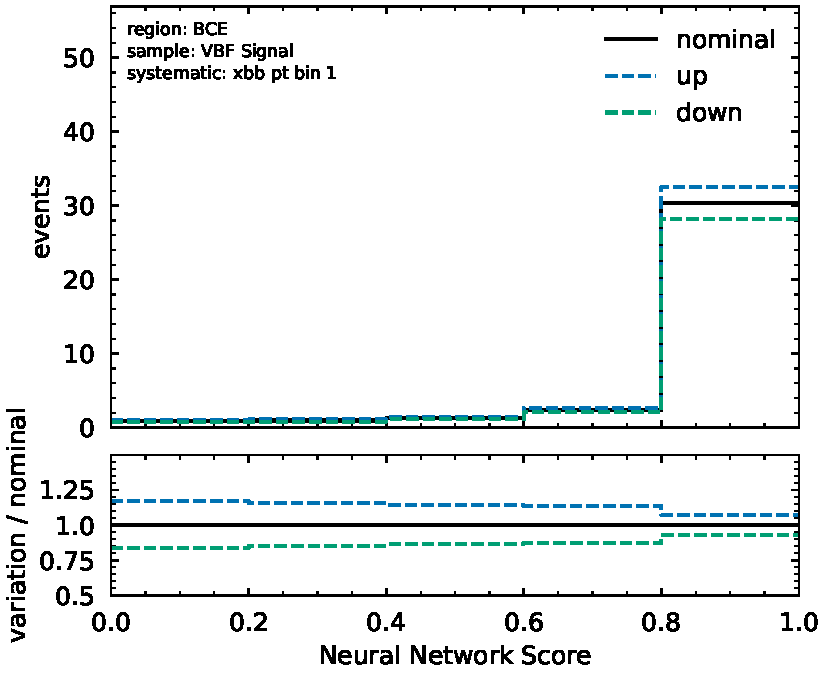
\includegraphics[width=.3\textwidth]{neos_results/tomatos_bce_5_1000_l1cvv0cv1/figures/templates/BCE_VBF-Signal_xbb-pt-bin-1.pdf}}
    \subfigure[]{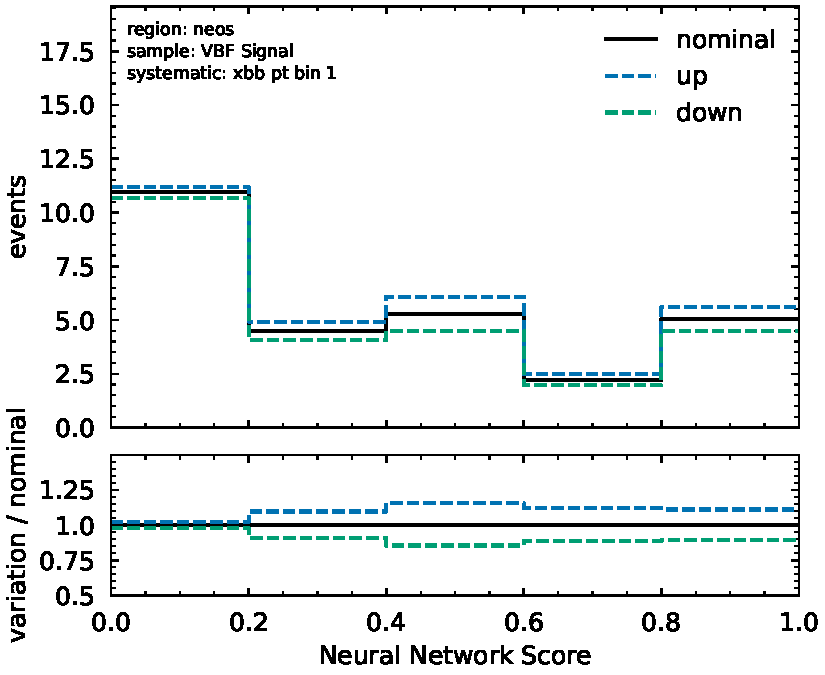
\includegraphics[width=.3\textwidth]{neos_results/tomatos_cls_5_2500_slope_50_l1cvv0cv1/figures/templates/neos_VBF-Signal_xbb-pt-bin-1.pdf}} \\
    \subfigure[]{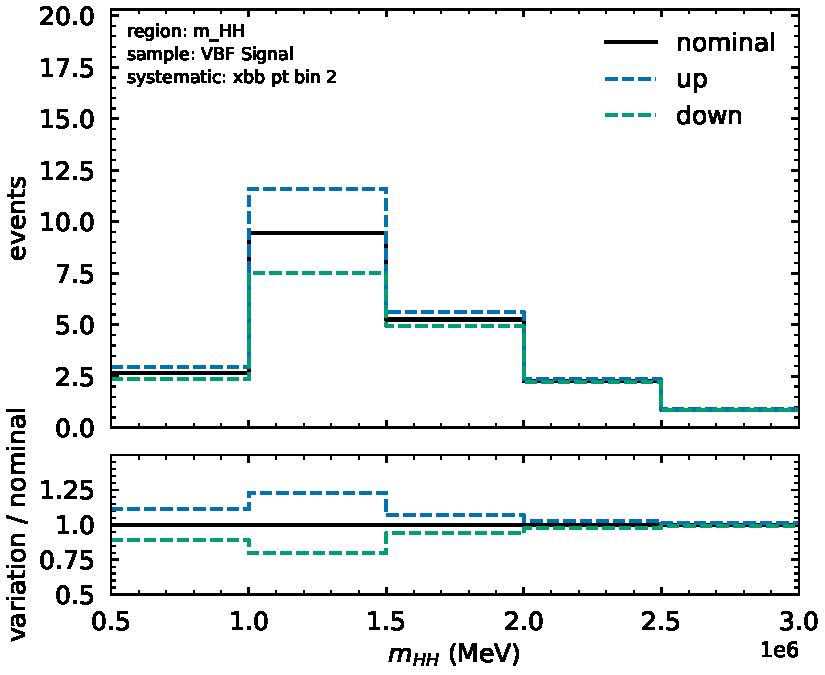
\includegraphics[width=.3\textwidth]{neos_results/m_hh_5_l1cvv0cv1/figures/templates/m_HH_VBF-Signal_xbb-pt-bin-2.pdf}}
    \subfigure[]{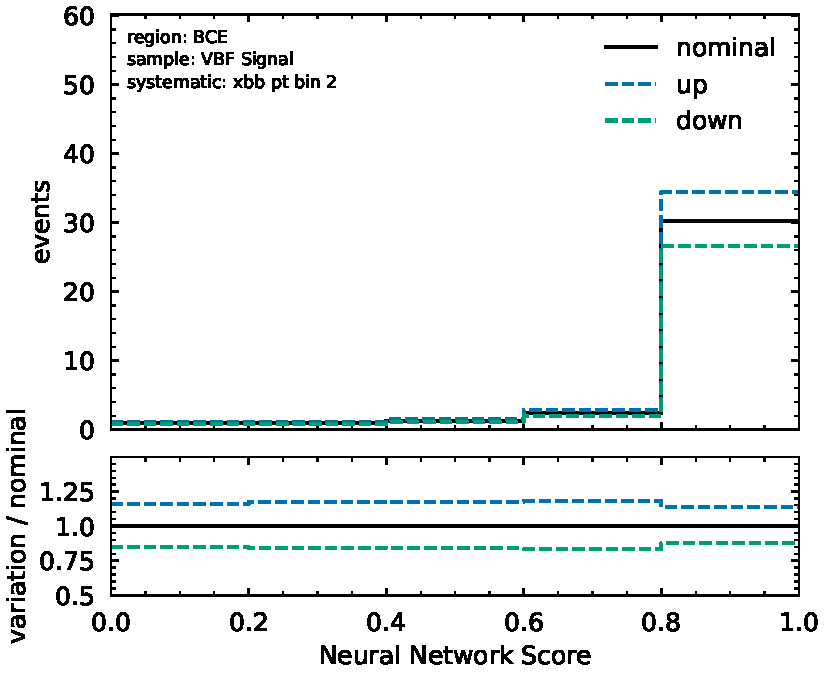
\includegraphics[width=.3\textwidth]{neos_results/tomatos_bce_5_1000_l1cvv0cv1/figures/templates/BCE_VBF-Signal_xbb-pt-bin-2.pdf}}
    \subfigure[]{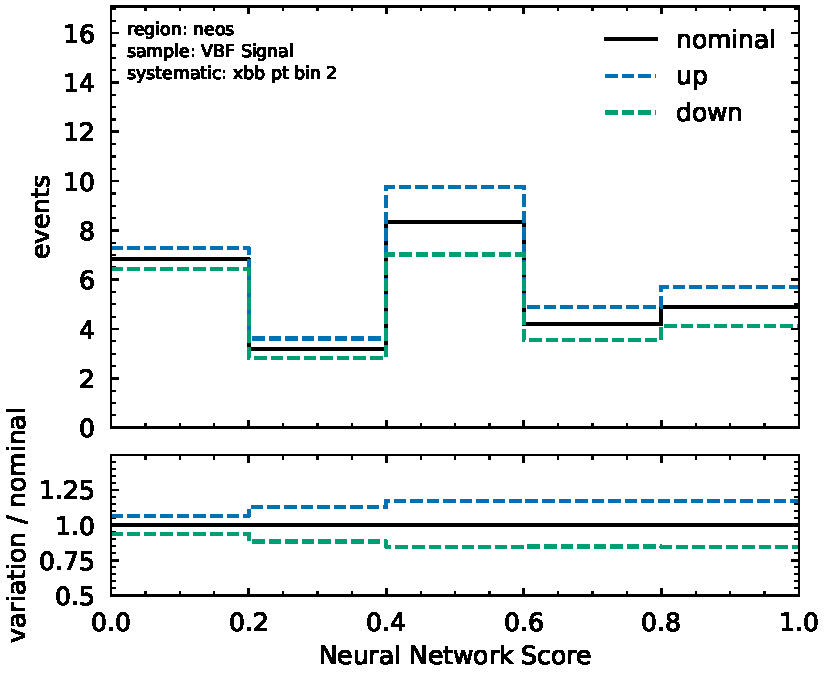
\includegraphics[width=.3\textwidth]{neos_results/tomatos_cls_5_2500_slope_50_l1cvv0cv1/figures/templates/neos_VBF-Signal_xbb-pt-bin-2.pdf}} \\
    \subfigure[]{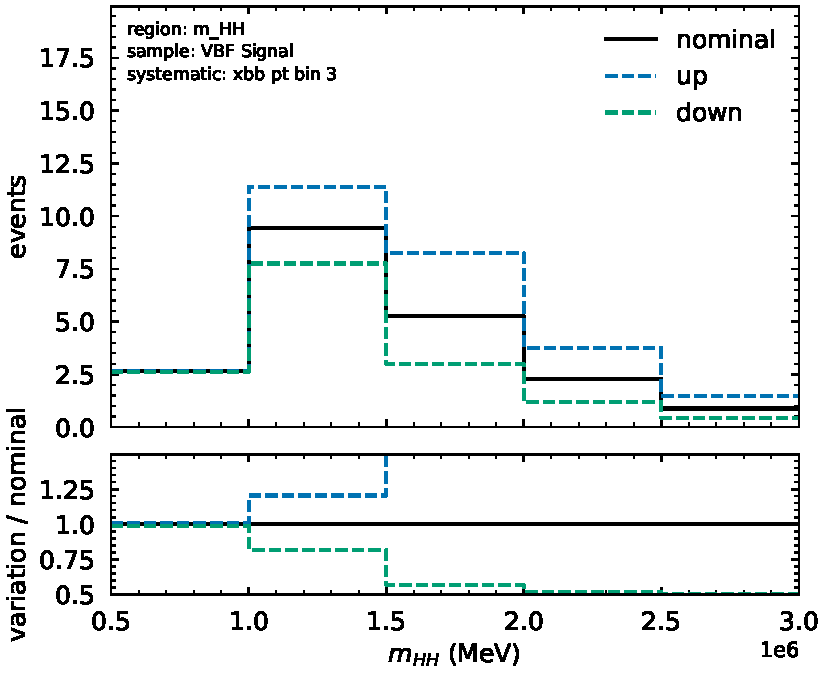
\includegraphics[width=.3\textwidth]{neos_results/m_hh_5_l1cvv0cv1/figures/templates/m_HH_VBF-Signal_xbb-pt-bin-3.pdf}}
    \subfigure[]{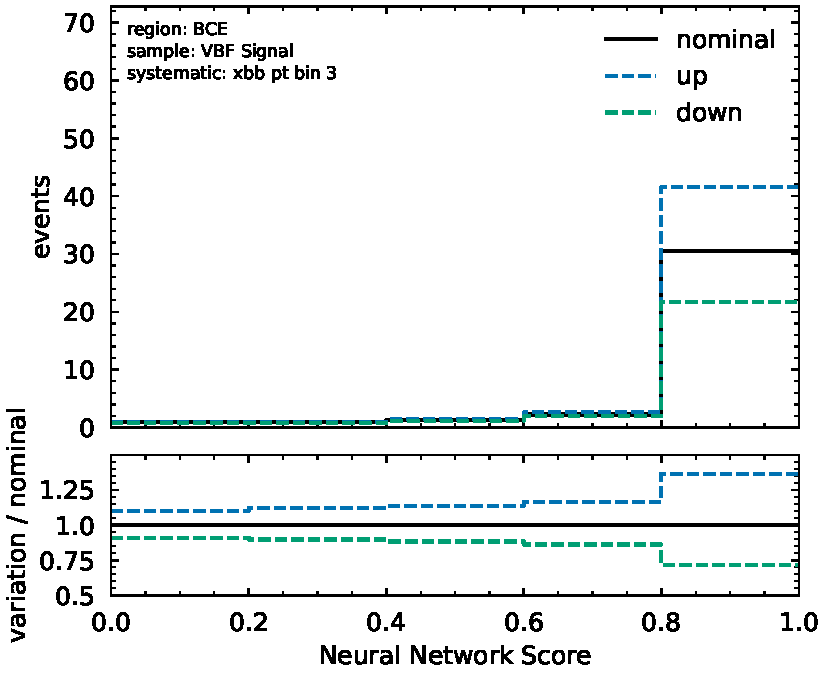
\includegraphics[width=.3\textwidth]{neos_results/tomatos_bce_5_1000_l1cvv0cv1/figures/templates/BCE_VBF-Signal_xbb-pt-bin-3.pdf}}
    \subfigure[]{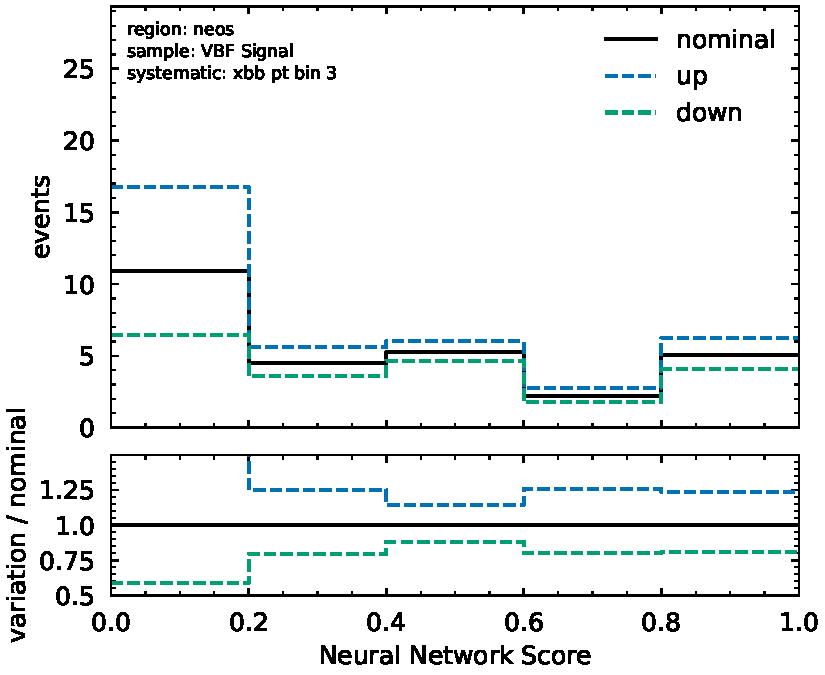
\includegraphics[width=.3\textwidth]{neos_results/tomatos_cls_5_2500_slope_50_l1cvv0cv1/figures/templates/neos_VBF-Signal_xbb-pt-bin-3.pdf}} \\
    \caption[]{Uncertainties (1/2) for columns left to right: $\mhh$, \ac{bce}-trained \ac{nn}, \ac{neos}-trained \ac{nn}. Top to bottom: 30\% GN2X scale factor uncertainties for the four bins used in the calibration of the GN2X tagger as shown in figure \ref{fig:xbb_sf}.\red{increase labels}}
    \label{fig:neos_validation_uncertaintes_1}
\end{figure}
\begin{figure}
    \centering
    \subfigure[]{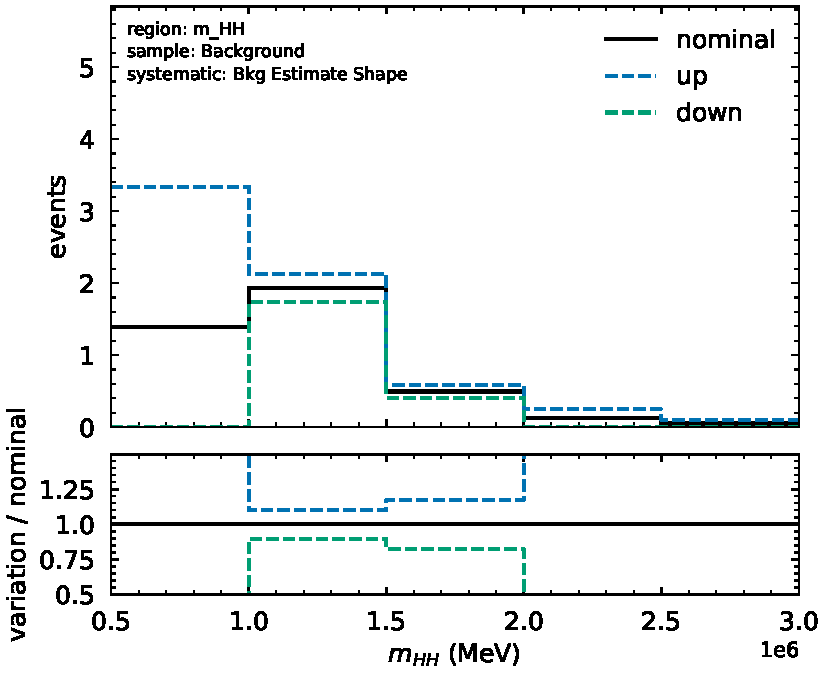
\includegraphics[width=.3\textwidth]{neos_results/m_hh_5_l1cvv0cv1/figures/templates/m_HH_Background_Bkg-Estimate-Shape.pdf}}   
    \subfigure[]{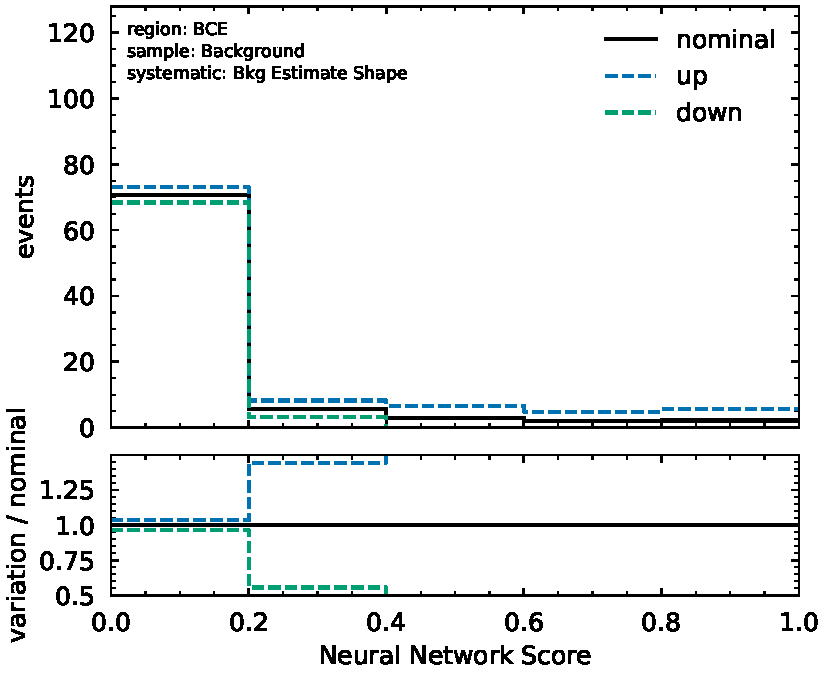
\includegraphics[width=.3\textwidth]{neos_results/tomatos_bce_5_1000_l1cvv0cv1/figures/templates/BCE_Background_Bkg-Estimate-Shape.pdf}}
    \subfigure[]{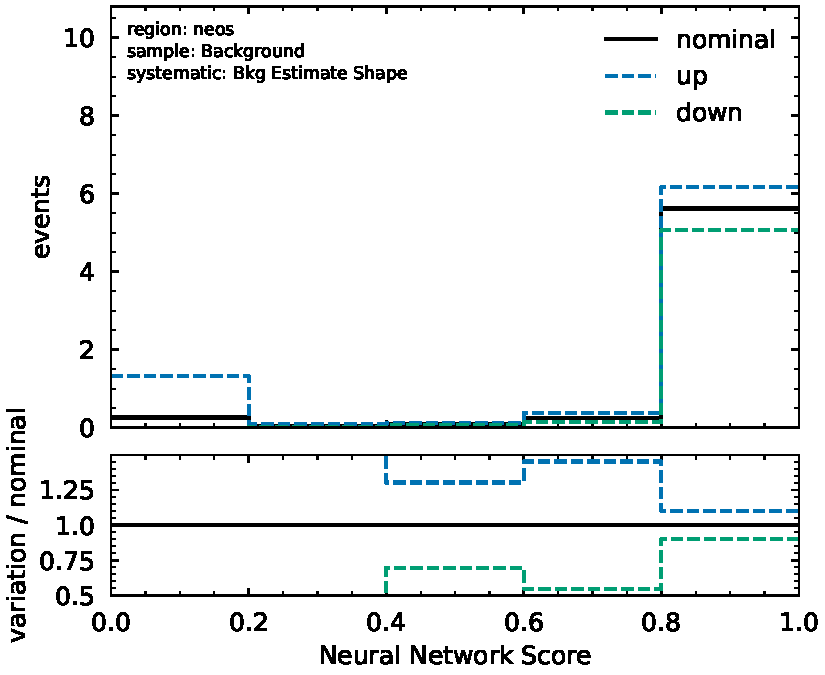
\includegraphics[width=.3\textwidth]{neos_results/tomatos_cls_5_2500_slope_50_l1cvv0cv1/figures/templates/neos_Background_Bkg-Estimate-Shape.pdf}} \\
    \subfigure[]{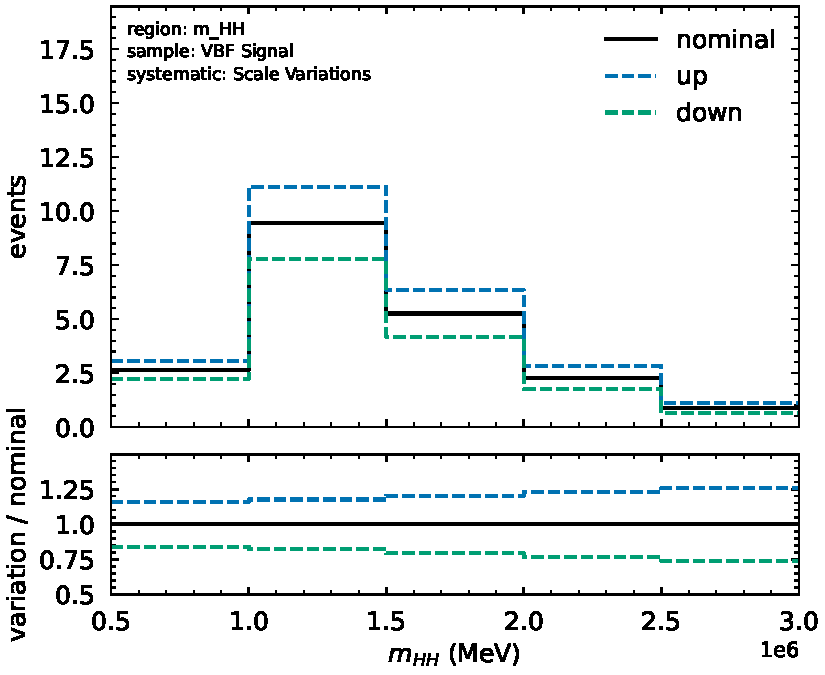
\includegraphics[width=.3\textwidth]{neos_results/m_hh_5_l1cvv0cv1/figures/templates/m_HH_VBF-Signal_Scale-Variations.pdf}}
    \subfigure[]{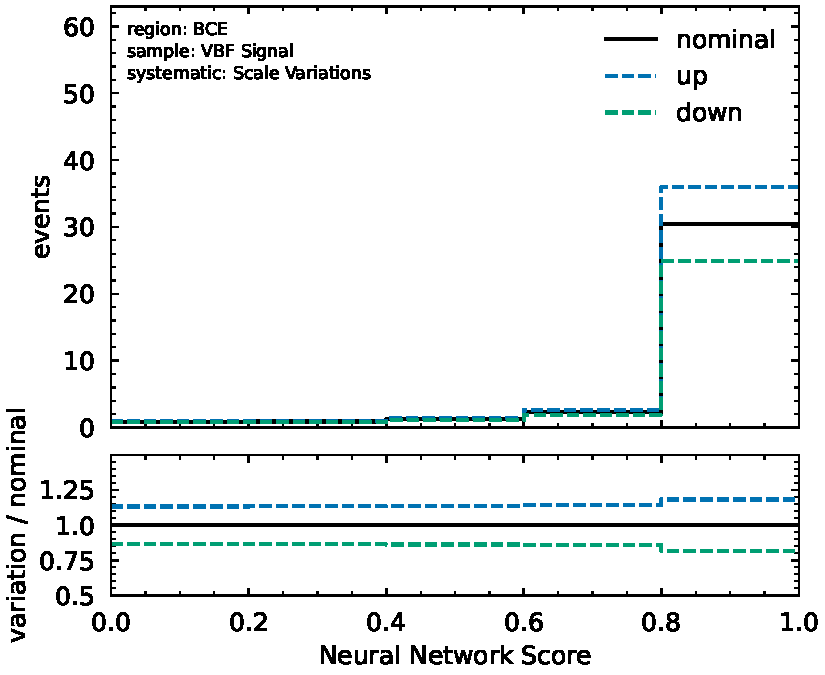
\includegraphics[width=.3\textwidth]{neos_results/tomatos_bce_5_1000_l1cvv0cv1/figures/templates/BCE_VBF-Signal_Scale-Variations}}
    \subfigure[]{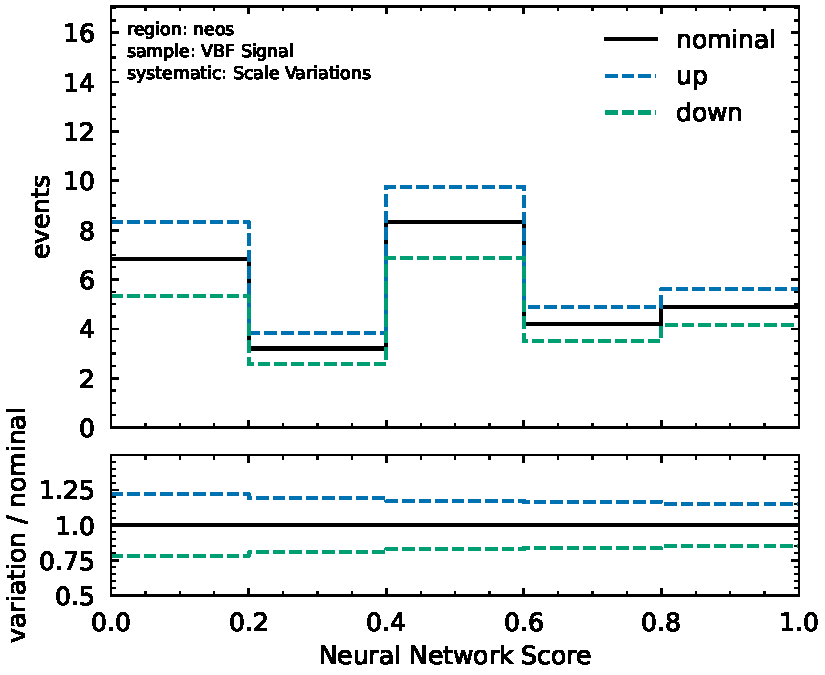
\includegraphics[width=.3\textwidth]{neos_results/tomatos_cls_5_2500_slope_50_l1cvv0cv1/figures/templates/neos_VBF-Signal_Scale-Variations.pdf}} \\
    \caption[]{Uncertainties (2/2) for columns left to right: $\mhh$, \ac{bce}-trained \ac{nn}, \ac{neos}-trained \ac{nn}. Top to bottom: background shape uncertainty and the envelope of scale variations. Details about their estimation are found in chapter \ref{ch:systematics}. \red{check again if these contain all} }
    \label{fig:neos_validation_uncertaintes_2}
\end{figure}

Histograms and their uncertainties are shown in figure \ref{fig:neos_pre_post_fit} before and after fitting. All models display more constrained postfit uncertainties.
\begin{figure}
    \centering
    \subfigure[]{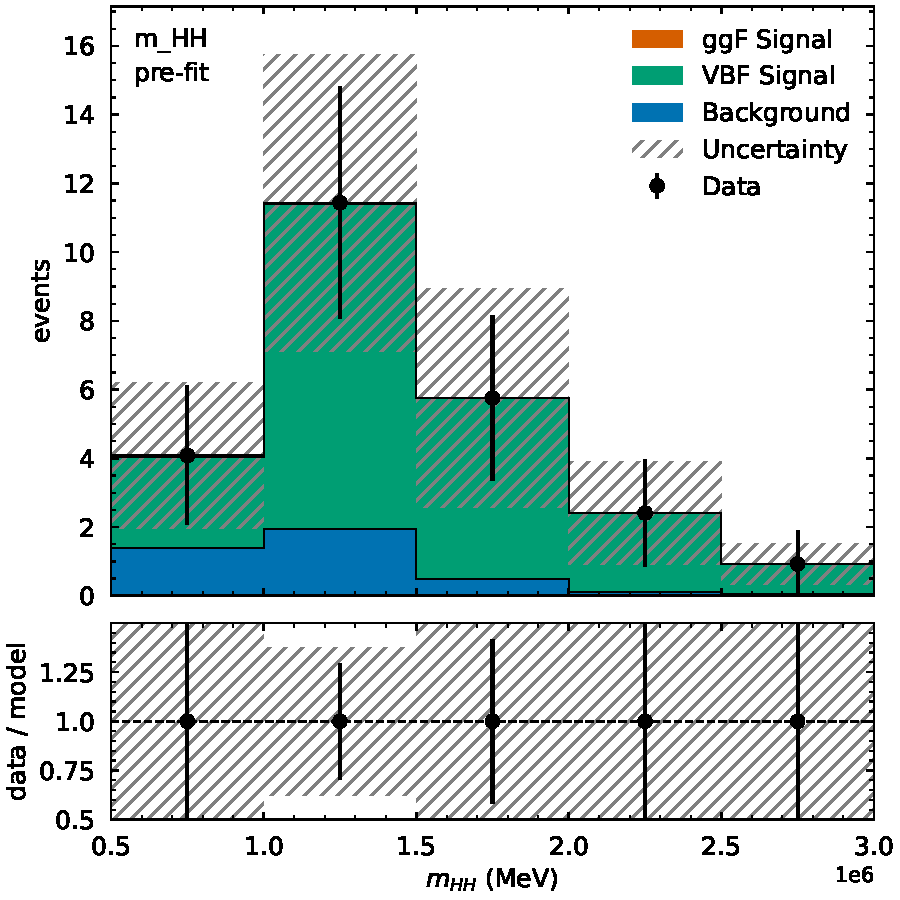
\includegraphics[width=.3\textwidth]{neos_results/m_hh_5_l1cvv0cv1/figures/m_HH_prefit.pdf}}
    \subfigure[]{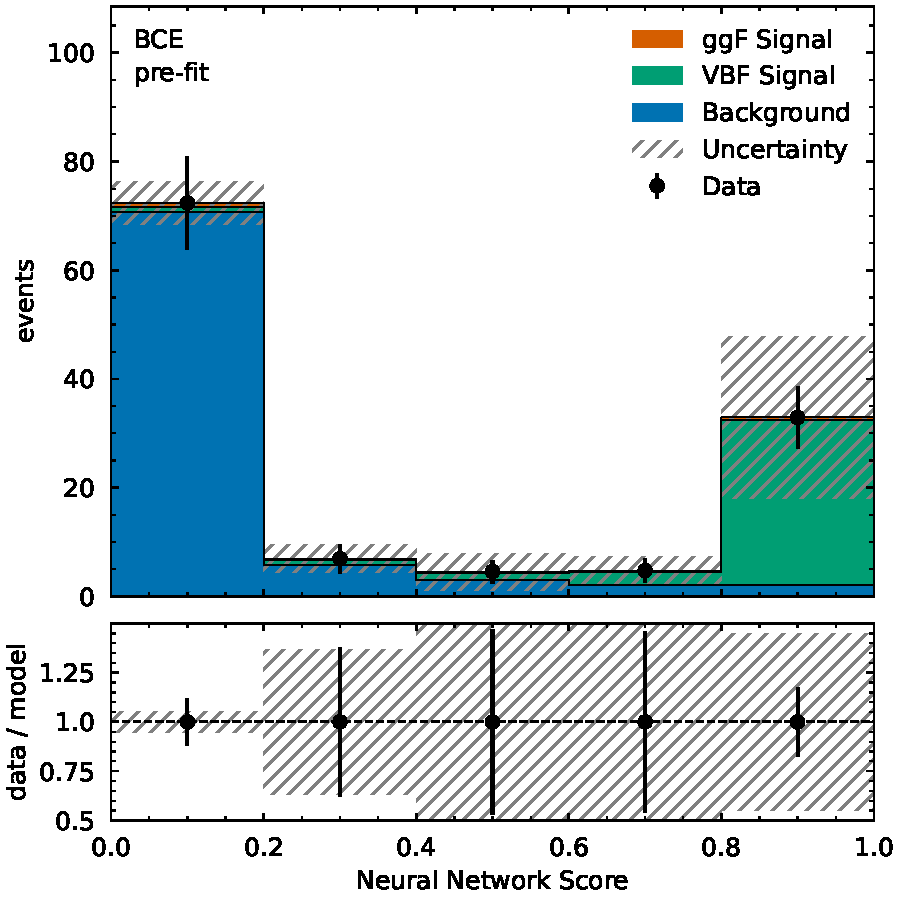
\includegraphics[width=.3\textwidth]{neos_results/tomatos_bce_5_1000_l1cvv0cv1/figures/BCE_prefit.pdf}}
    \subfigure[]{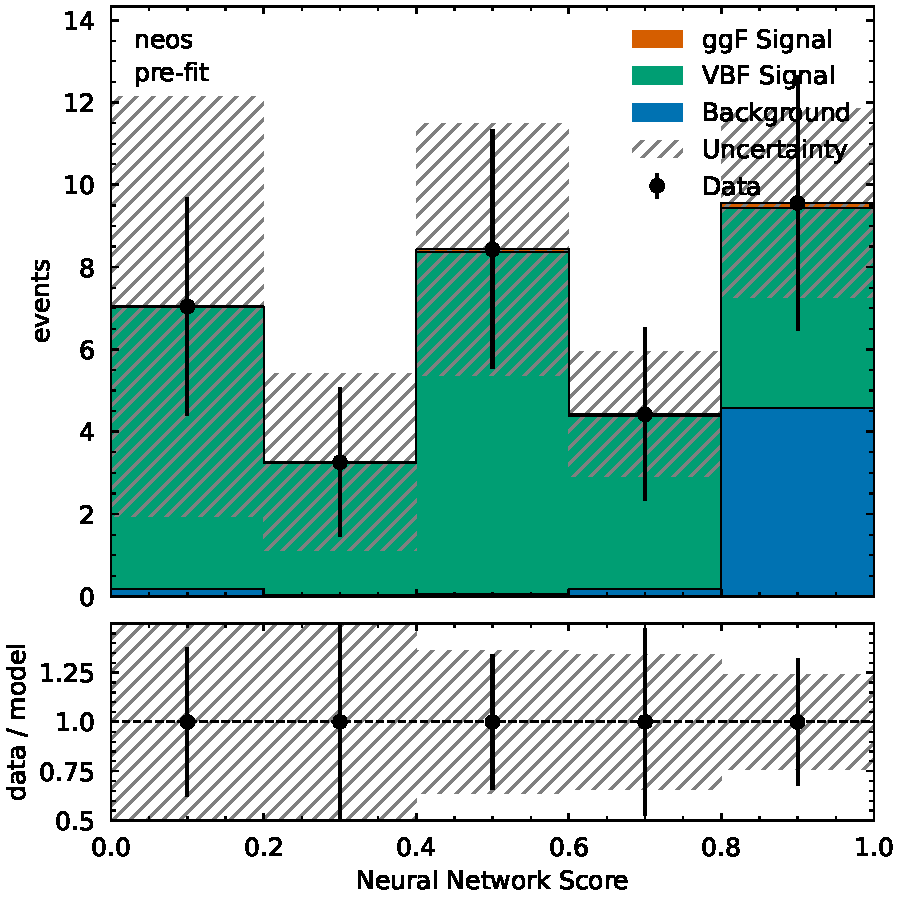
\includegraphics[width=.3\textwidth]{neos_results/tomatos_cls_5_2500_slope_50_l1cvv0cv1/figures/neos_prefit.pdf}} \\
    \subfigure[]{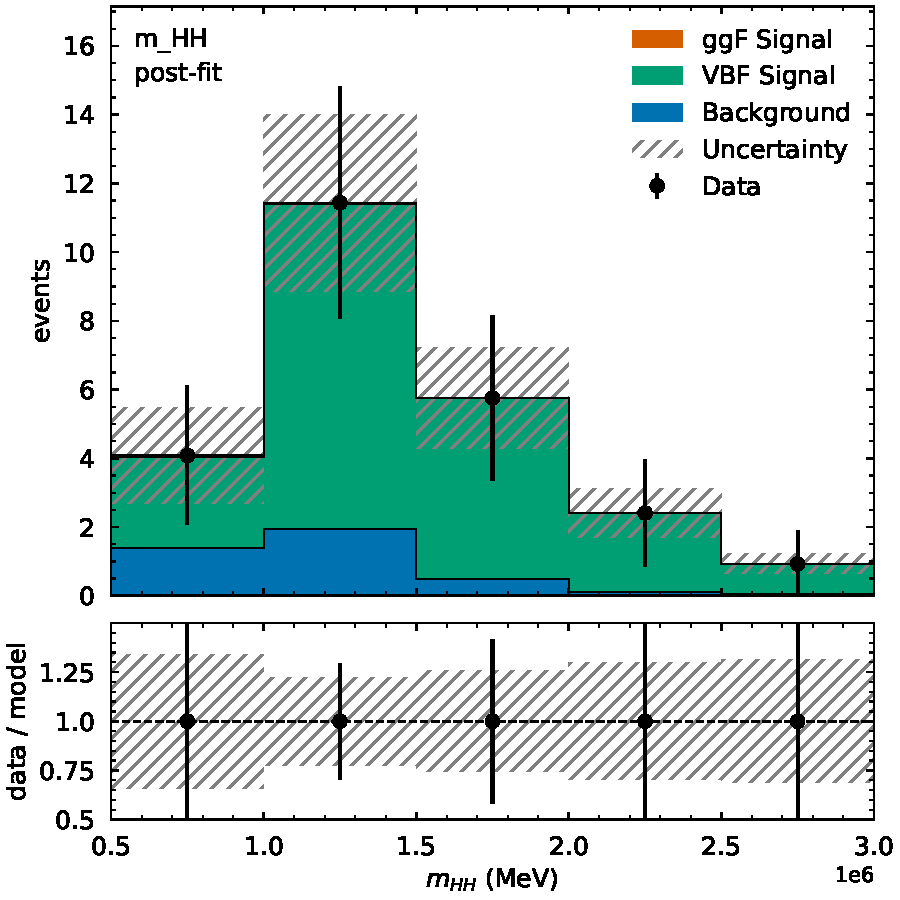
\includegraphics[width=.3\textwidth]{neos_results/m_hh_5_l1cvv0cv1/figures/m_HH_postfit.pdf}}
    \subfigure[]{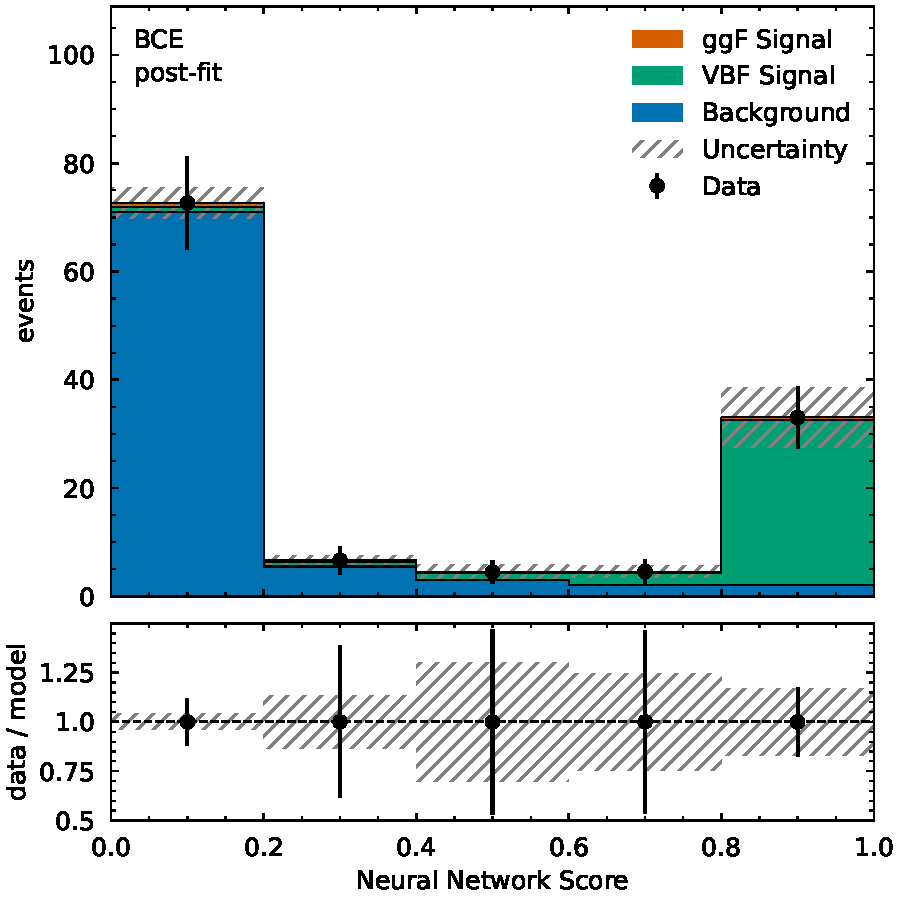
\includegraphics[width=.3\textwidth]{neos_results/tomatos_bce_5_1000_l1cvv0cv1/figures/BCE_postfit.pdf}}
    \subfigure[]{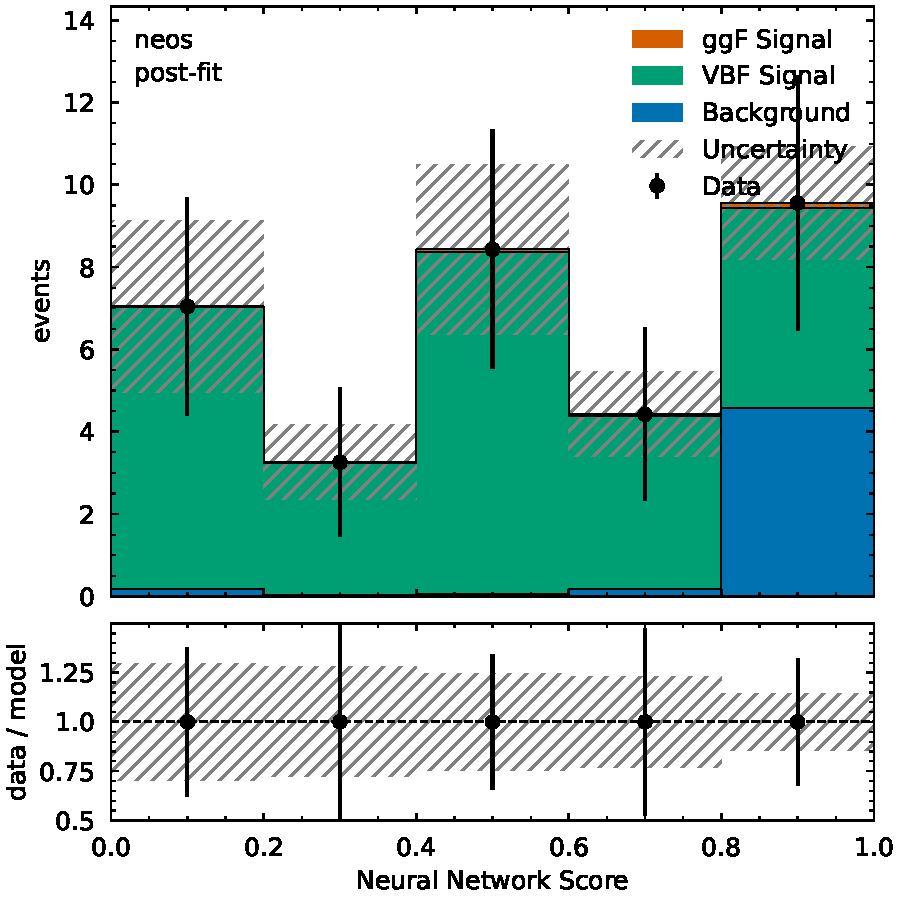
\includegraphics[width=.3\textwidth]{neos_results/tomatos_cls_5_2500_slope_50_l1cvv0cv1/figures/neos_postfit.pdf}}
    \caption[]{Pre- \textbf{(a)-(c)} and Postfit \textbf{(d)-(f)} histogram for columns left to right: $\mhh$, \ac{bce}-trained \ac{nn}, \ac{neos}-trained \ac{nn} }
    \label{fig:neos_pre_post_fit}
\end{figure}

Nuisance parameter rankings for the \ac{bce}-trained and neos-trained \ac{nn} are shown in figure \ref{fig:neos_valid_ranking_bce} and \ref{fig:neos_valid_ranking_cls}. Since \ac{neos} optimizes on the fitting procedure, nuisance parameter pre- and postfit impacts are generally smaller compared to the \ac{bce}-trained \ac{nn}. The dominating uncertainties are generally in this analysis the GN2X version of the $X\rightarrow bb$ tagger and the scale variations, detailed in chapter \ref{ch:systematics}. The most prominent feature of \ac{neos} in this analysis is its ability to adjust the \ac{nn} with respect to the background estimate moving it in the ranking even below the dominating uncertainties. In turn the \ac{bce}-trained \ac{nn} shows that the background estimate uncertainty is overestimated pre-fitting as the impacts on the signal strength and a small pull uncertainty reveals.

\begin{figure}
    \centering
    \includegraphics[width=1\textwidth]{neos_results/tomatos_bce_5_1000_l1cvv0cv1/figures/ranking.pdf}
    \caption[]{Ranking of nuisance parameters ordered by their post-fit impact on the signal strength, $\Delta\mu$, displayed on the upper axis for the \ac{bce}-trained \ac{nn}. The black dots and the lower axis represent the pulls. A detailed explanation of this plot can be found in figure \ref{fig:m_hh_neos_unc_ranking}.}
    \label{fig:neos_valid_ranking_bce}
\end{figure}
\begin{figure}
    \centering
    \includegraphics[width=1\textwidth]{neos_results/tomatos_cls_5_2500_slope_50_l1cvv0cv1/figures/ranking.pdf}
    \caption[]{Ranking of nuisance parameters ordered by their post-fit impact on the signal strength, $\Delta\mu$, displayed on the upper axis for \ac{neos}. The black dots and the lower axis represent the pulls. A detailed explanation of this plot can be found in figure \ref{fig:m_hh_neos_unc_ranking}.}
    \label{fig:neos_valid_ranking_cls}
\end{figure}

Furthermore the correlation matrices for the models in figures \ref{fig:correlation_matrix_m_hh}, \ref{fig:correlation_matrix_bce} and \ref{fig:correlation_matrix_cls} reveal a strong correlation of the signal strength to the uncertainties of the GN2X version of the $X\rightarrow bb$ tagger. When propagating errors, covariances contribute to the overall uncertainty. This can be understood by examining the variance of a function $f(\theta_1, \theta_2)$ depending on two parameters with their individual $\sigma_1,\sigma_2$ uncertainties
\begin{equation}
    \text{Var}(f(\theta_1, \theta_2)) = \left( \frac{\partial f}{\partial \theta_1} \right)^2 \sigma_1^2 + \left( \frac{\partial f}{\partial \theta_2} \right)^2 \sigma_2^2 + 2 \left( \frac{\partial f}{\partial \theta_1} \right) \left( \frac{\partial f}{\partial \theta_2} \right) \sigma_{12}.
\end{equation}
Thus, if parameters $\theta_1, \theta_2$ are correlated the cross-term \(2 \left( \frac{\partial f}{\partial \theta_1} \right) \left( \frac{\partial f}{\partial \theta_2} \right) \sigma_{12}\) contributes to the overall uncertainty. \ac{neos} appears to have the capability to decorrelate uncertainties, thereby potentially reducing the impact of these correlated uncertainties on the overall analysis. \red{ist das zu mutmaßlich, wir sehen das zwar, aber es ist kein beweis.}

\begin{figure}
    \centering
    \includegraphics[width=1\textwidth]{neos_results/m_hh_5_l1cvv0cv1/figures/correlation_matrix.pdf}
    \caption[]{Correlation matrix of correlation coefficients between parameters for \mhh.}
    \label{fig:correlation_matrix_m_hh}
\end{figure}
\begin{figure}
    \centering
    \includegraphics[width=1\textwidth]{neos_results/tomatos_bce_5_1000_l1cvv0cv1/figures/correlation_matrix.pdf}
    \caption[]{Correlation matrix of correlation coefficients between parameters for the \ac{bce}-trained \ac{nn}.}
    \label{fig:correlation_matrix_bce}
\end{figure}
\begin{figure}
    \centering
    \includegraphics[width=1\textwidth]{neos_results/tomatos_cls_5_2500_slope_50_l1cvv0cv1/figures/correlation_matrix.pdf}
    \caption[]{Correlation matrix of correlation coefficients between parameters for \ac{neos}.}
    \label{fig:correlation_matrix_cls}
\end{figure}

Expected limits on the cross-section for $\ktwov=0$ and the \ac{sm} \ac{vbf} signal are shown in figure \ref{fig:neos_valid_brazil_limits}. For the $\ktwov=0$ signal the relative improvement of the \ac{neos} approach compared to \mhh is about \qty[]{35}{\percent} whereas in relation to the \ac{bce}-trained \ac{nn} the improvement linearly ranges between \qty[]{5}{\percent} and \qty[]{20}{\percent} with a nominal expected limit improvement of \qty[]{10}{\percent} as shown in figure \ref{fig:neos_valid_brazil_limits}(c). Decreased performance of \ac{neos} evaluated on the \ac{sm} signal suggests that when using neos results could benefit from a retraining/reoptimization for different \ktwov hypotheses.
\begin{figure}
    \centering
    \subfigure[]{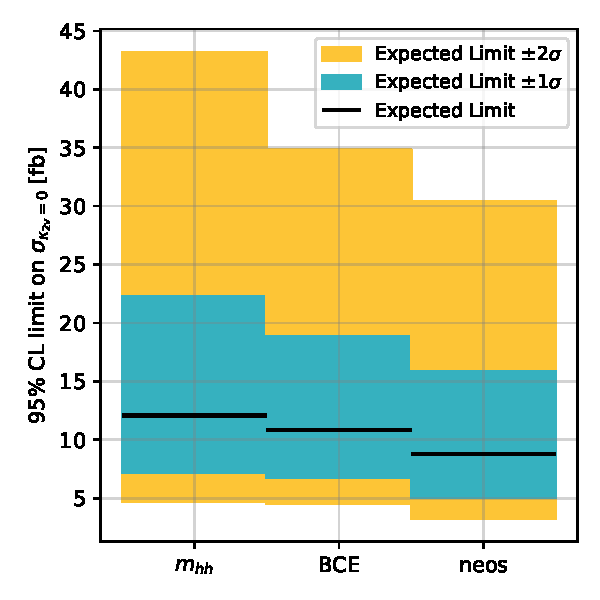
\includegraphics[width=.47\textwidth]{neos_results/brazil_limits_k2v0.pdf}}
    \subfigure[]{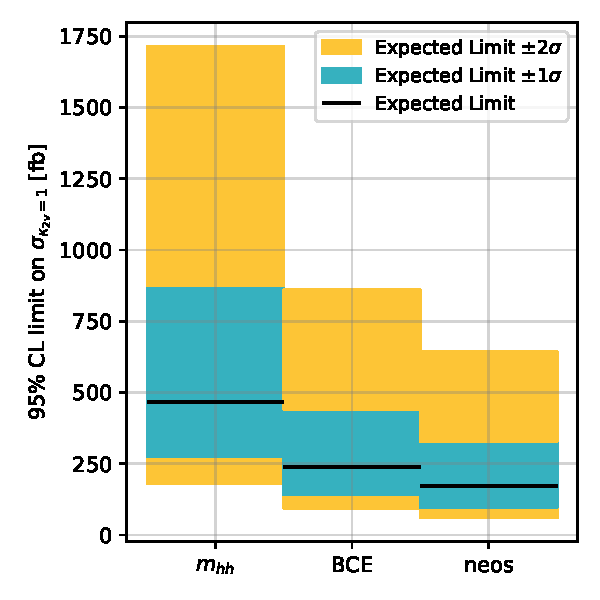
\includegraphics[width=.47\textwidth]{neos_results/brazil_limits_k2v1.pdf}}\\
    \subfigure[]{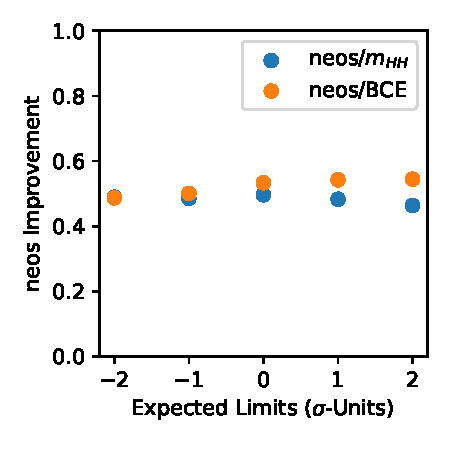
\includegraphics[width=.4\textwidth]{neos_results/relative_limits_k2v0.pdf}}
    \caption[]{Cross-sectional limits on the nominal (a) \ac{vbf} $\ktwov=0$ and (b) \ac{sm} \ac{vbf} $\ktwov=1$ signal. (c) Relative improvements on expected limits of neos to $m_{HH}$ and the \ac{bce}-trained model for the $\ktwov=0$ signal hypothesis.}
    \label{fig:neos_valid_brazil_limits}
\end{figure}

With the linear combination of \ac{vbf} signal hypotheses as explained in section \ref{sec:linear_combination} a \ktwov scan for the three models is conducted with determined limits shown in figure \ref{fig:neos_valid_k2v_scan}. The constrained limits for \ktwov are summed up in table \ref{tab:neos_valid_k2v_constraints} with a relative improvement of neos to \ac{bce}-trained \ac{nn} (\mhh) of \qty[]{10}{(27)\percent} on the lower limit and \qty[]{3}{(9)\percent}.
\red{show overlay here, in final part only brazil scan}



\begin{figure}
    \centering
    \subfigure[]{\includegraphics[width=.3\textwidth]{neos_results/m_hh_5_nominal_reweighted_ratio}}
    \subfigure[]{\includegraphics[width=.3\textwidth]{neos_results/tomatos_bce_5_1000_nominal_reweighted_ratio}}
    \subfigure[]{\includegraphics[width=.3\textwidth]{neos_results/tomatos_cls_5_2500_slope_50_nominal_reweighted_ratio}} \\
    \caption[]{\red{maybe in appendix?}}
    \label{fig:reweight_validation}
\end{figure}




\begin{figure}
    \centering
    \includegraphics[width=1\textwidth]{neos_results/k2v_scan_limits_overlay_neos_validation.pdf}
    \caption[]{Expected cross-section limits depending on \ktwov for the three models.}
    \label{fig:neos_valid_k2v_scan}
\end{figure}
\begin{table}[htbp]\label{tab:neos_valid_k2v_constraints}
    \centering
    \caption{Expected constraints on \ktwov for the three models.}
    \begin{tabular}{c|c|c}
                                  & Lower \ktwov Limit & Upper \ktwov Limit \\\hline
        \mhh                      & 0.37               & 1.65               \\
        \ac{bce}-trained \ac{nn}  & 0.46               & 1.57               \\
        \ac{neos}-trained \ac{nn} & 0.51               & 1.52               \\
    \end{tabular}
\end{table}

\red{maybe move this to discussion}
This highlights the crux of the situation as optimizing on Asimov significance alone cannot account for uncertainties and has thus decreased performance compared to \ac{neos}. If \ac{neos} is not applicable it can be advisable when searching for a new process to implement a loss function that optimizes the Asimov significance given the observed correlation in figure \ref{fig:neos_validation_loss}. A study on this has also shown that such an approach can give improved results for analyses dominated by systematic uncertainties \citep{elwood2018direct}.
